\chapter{Introduzione}
\label{chap:introduzione}

\begin{figure}[H]
    \centering
    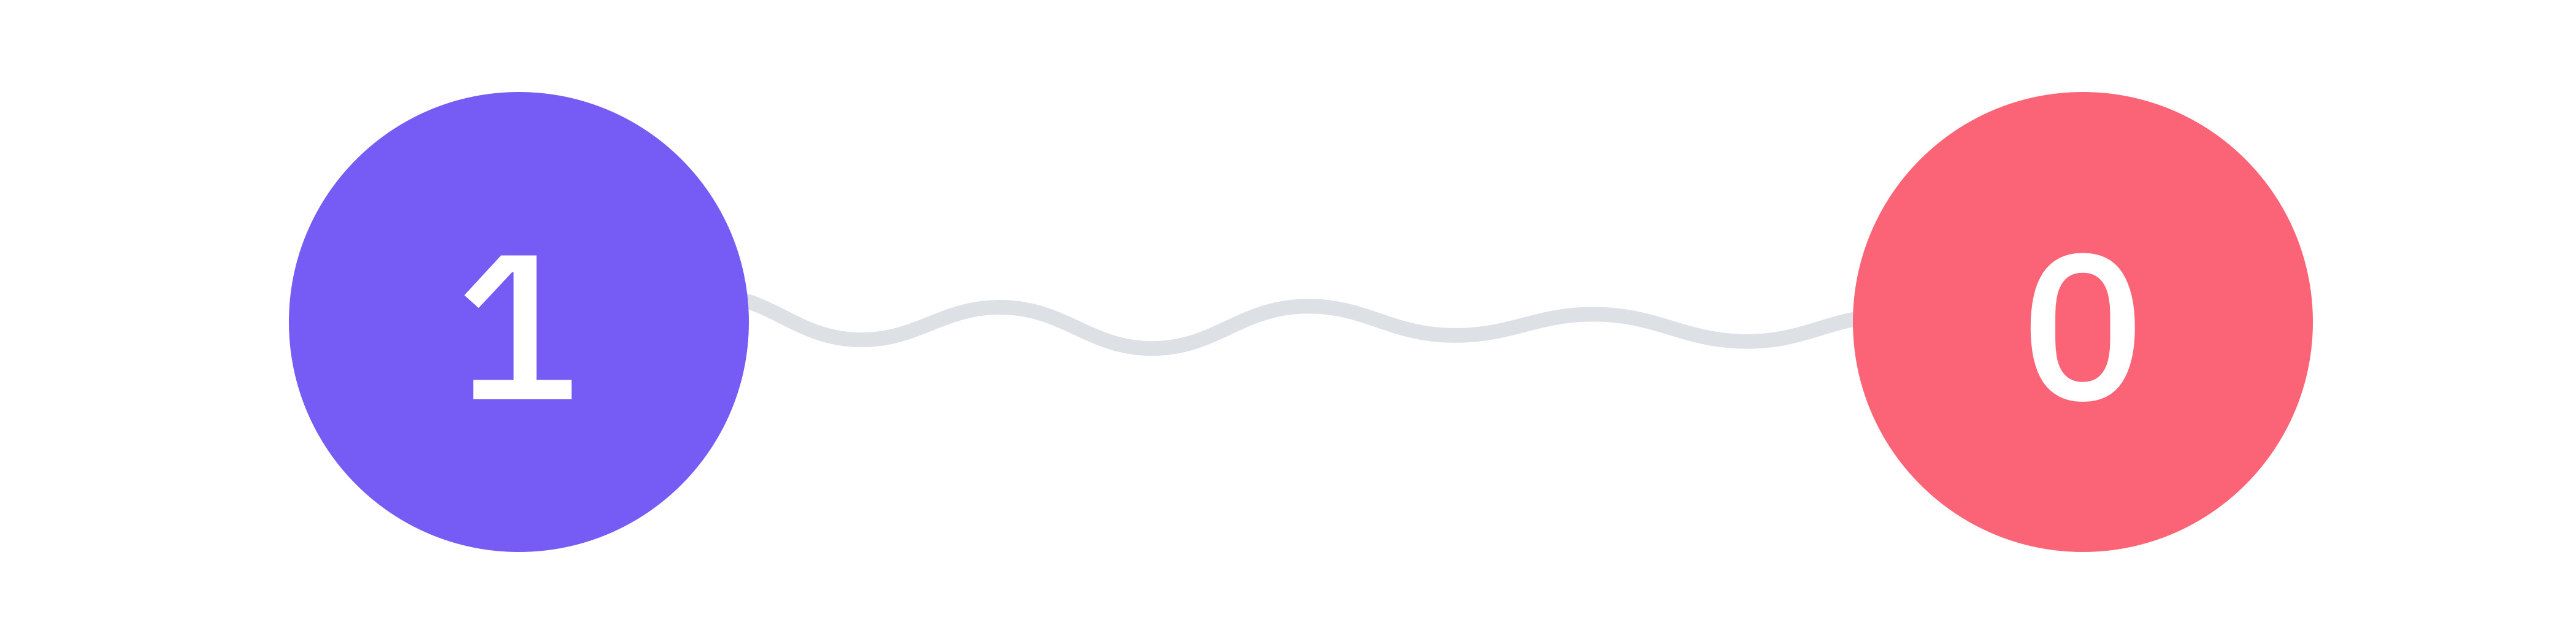
\includegraphics[alt={Testo alternativo dell'immagine}, width=1\columnwidth]{img/quantum_entanglement.jpeg}
    \caption{Lorem}
    \label{fig:entanglement}
\end{figure}

Introduzione al contesto applicativo.

Lorem Figure \ref{fig:entanglement}

Esempio di utilizzo di un termine nel glossario \gls{api}.

Esempio di citazione in linea \cite{site:agile-manifesto}.

Esempio di citazione nel piè di pagina citazione\footcite{womak:lean-thinking}

\lipsum[1-2]

\section{L'azienda}
\lipsum[1]

\section{L'idea}
Introduzione all'idea dello stage\footcite{article:spooky}.
\lipsum[1-3]

\section{Organizzazione del testo}
\begin{description}
    \item[{\hyperref[chap:processi-metodologie]{Il secondo capitolo}}] descrive ...
    
    \item[{\hyperref[chap:descrizione-stage]{Il terzo capitolo}}] approfondisce ...
    
    \item[{\hyperref[chap:analisi-requisiti]{Il quarto capitolo}}] approfondisce ...
    
    \item[{\hyperref[chap:progettazione-codifica]{Il quinto capitolo}}] approfondisce ...
    
    \item[{\hyperref[chap:verifica-validazione]{Il sesto capitolo}}] approfondisce ...
    
    \item[{\hyperref[chap:conclusioni]{Nel settimo capitolo}}] descrive ...
\end{description}

Riguardo la stesura del testo, relativamente al documento sono state adottate le seguenti convenzioni tipografiche:
\begin{itemize}
	\item gli acronimi, le abbreviazioni e i termini ambigui o di uso non comune menzionati vengono definiti nel glossario, situato alla fine del presente documento;
	\item per la prima occorrenza dei termini riportati nel glossario viene utilizzata la seguente nomenclatura: \textit{parola}\glox\gloxspacing;
	\item i termini in lingua straniera o facenti parti del gergo tecnico sono evidenziati con il carattere \textit{corsivo}.
\end{itemize}

\begin{listing}[H]
\begin{minted}{c}
#include <stdio.h>
int main() {
    print("Hello, world!");
    return 0;
}
\end{minted}
\caption{Example of code}
\label{listing:a}
\end{listing}

\newpage